\documentclass{article}

\usepackage{amsmath}
\usepackage{graphicx}

\begin{document}
\title{MCMD w3 -- Protein Fibril Formation}
\author{Alex Arash Sand Kalaee\\ \texttt{kalaee@teorfys.lu.se}}
\maketitle
We compare the obtained estimates of $\ln g(E)$ for systems A (1D) and B (2D),
see Fig~\ref{fig:compar}, for the last five iterations in $f$ for each to
evaluate the convergence. From the figure we find that the estimates
have converged in both systems.

\begin{figure}
\centering
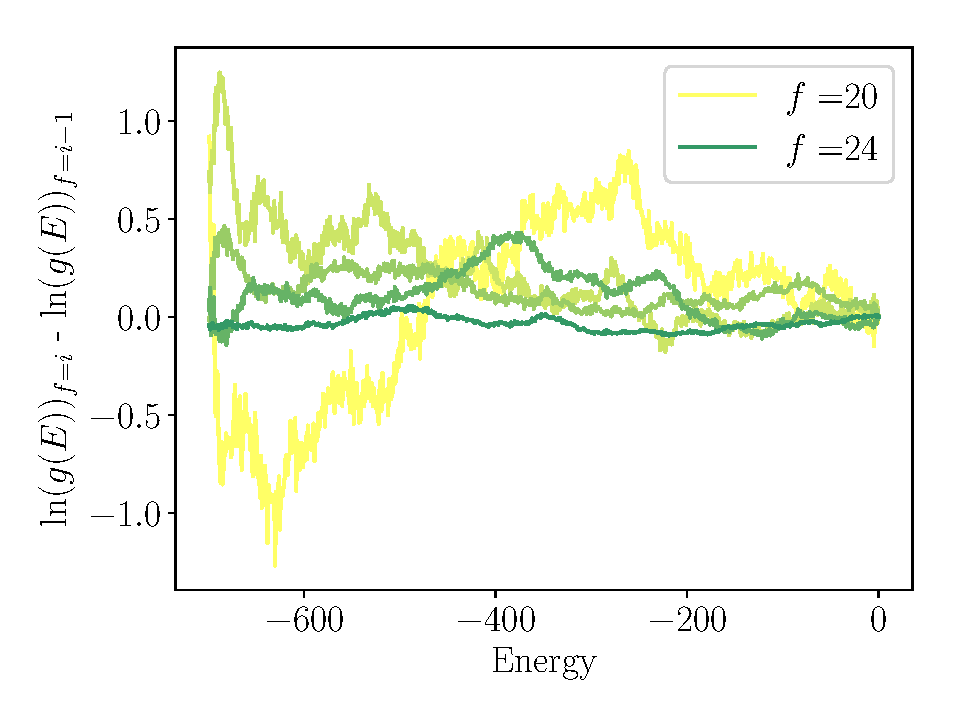
\includegraphics[width=0.49\linewidth]{projA_0.pdf}
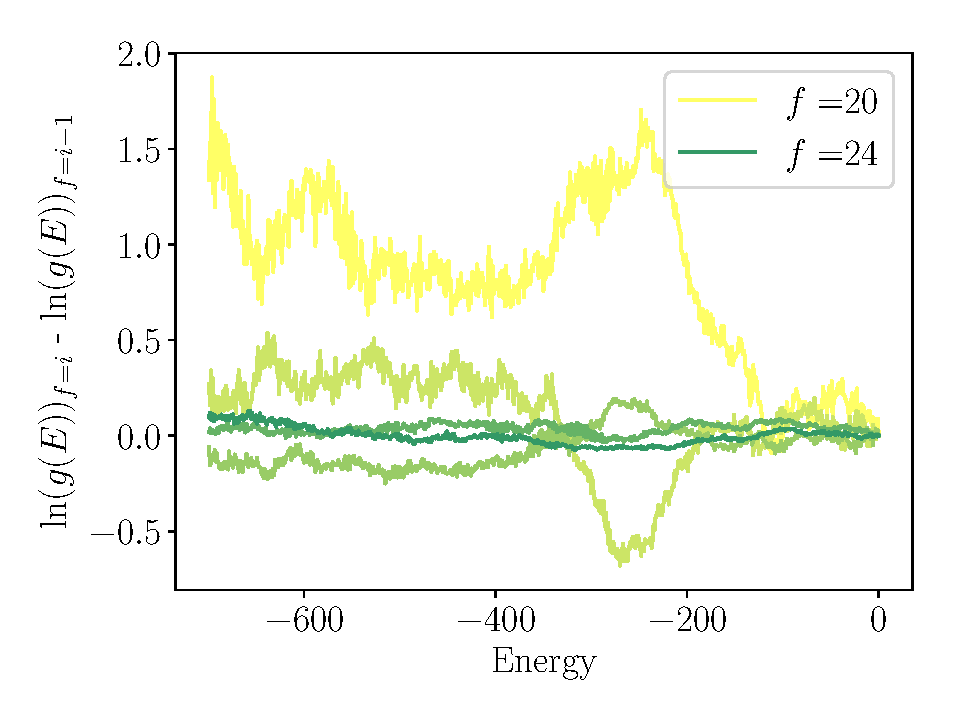
\includegraphics[width=0.49\linewidth]{projB_0.pdf}
\caption{ Difference between iterations for last five $f$-values in the
Wang-Landau estimation of $\ln g(E)$ for systems A (left) and B (right),
respectively. The colour changes from yellow to green as we convergence settles.}
\label{fig:compar}
\end{figure}

\section{Heat capacity}
Using the converged estimates for both systems we estimate the respective
heat capacities. Note that due to considerations of unphysical cyclical
aggregates we omit temperatures where the probabilities $P_T(E=-699)$ or
$P_T(E=-698)$ are above the threshold $10^{-4}$. The heat capacities
are provided in Fig.~\ref{fig:heat}. The heat capacity is maximised at the
points $T_A = 0.650$ for system A and $T_B= 0.657$ for B.

\begin{figure}
\centering
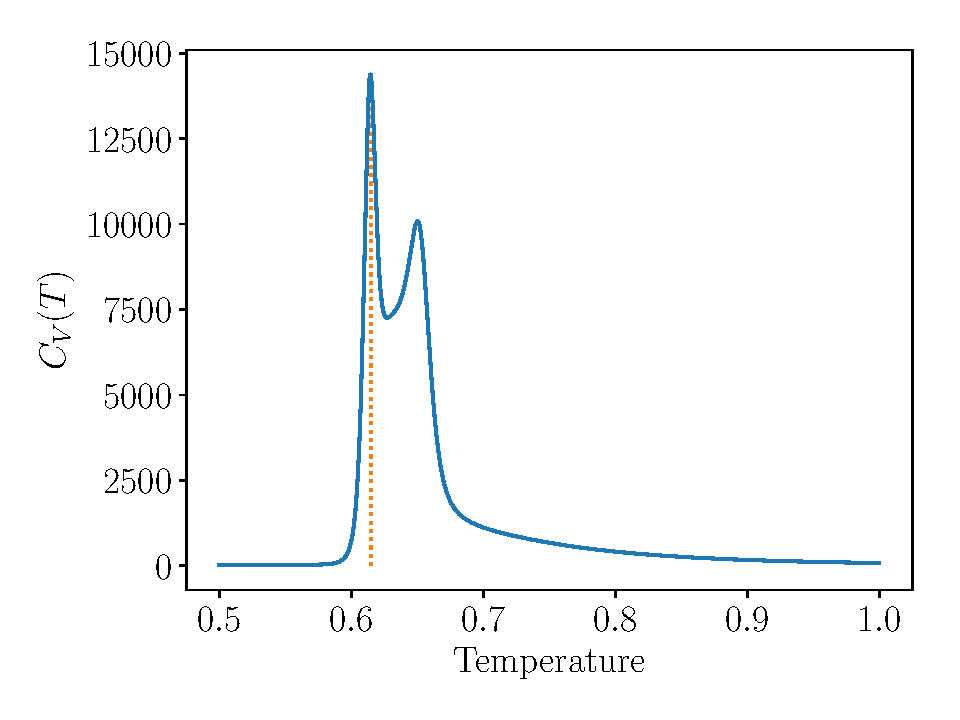
\includegraphics[width=0.49\linewidth]{projA_1.pdf}
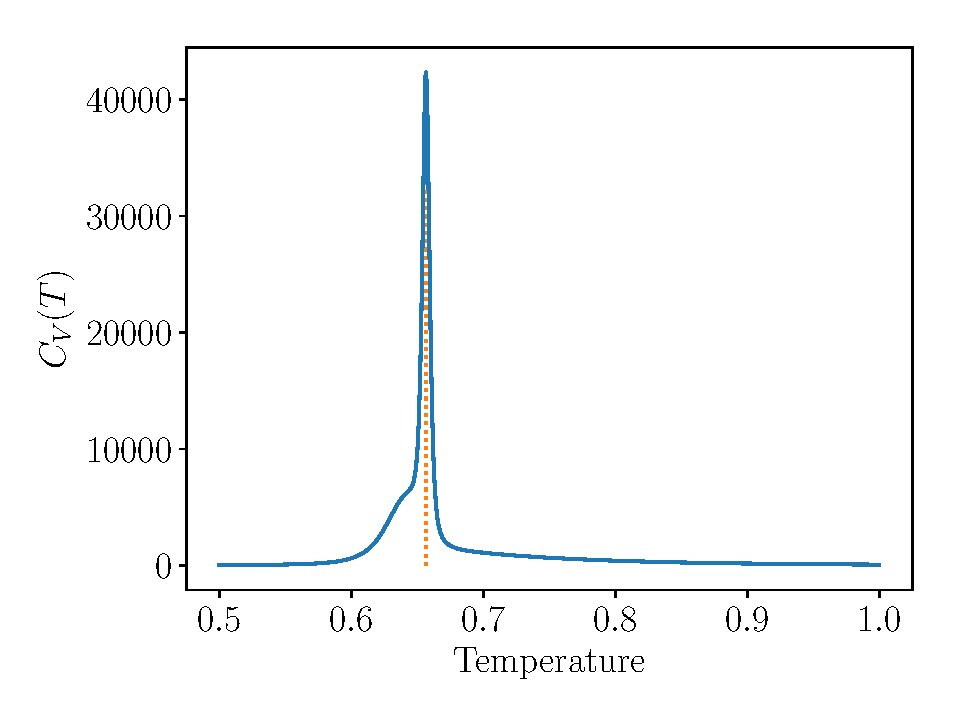
\includegraphics[width=0.49\linewidth]{projB_1.pdf}
\caption{Heat capacity for temperatures with physical solutions for system
A (left) and B (right)}
\label{fig:heat}
\end{figure}

\section{Probability distribution}
Finally, we construct the probability distribution functions (PDFs) for the
systems at the temperatures that maximises the respective heat capacities.
The data is smoothed in bins of width 4, see Fig~\ref{fig:pdf}.
For a system with an abrupt transition between the disordered solution
and the mixed state one expects a bimodal energy distribution. According
to the obtained PDFs system A is unimodal while B is bimodal.

\begin{figure}
\centering
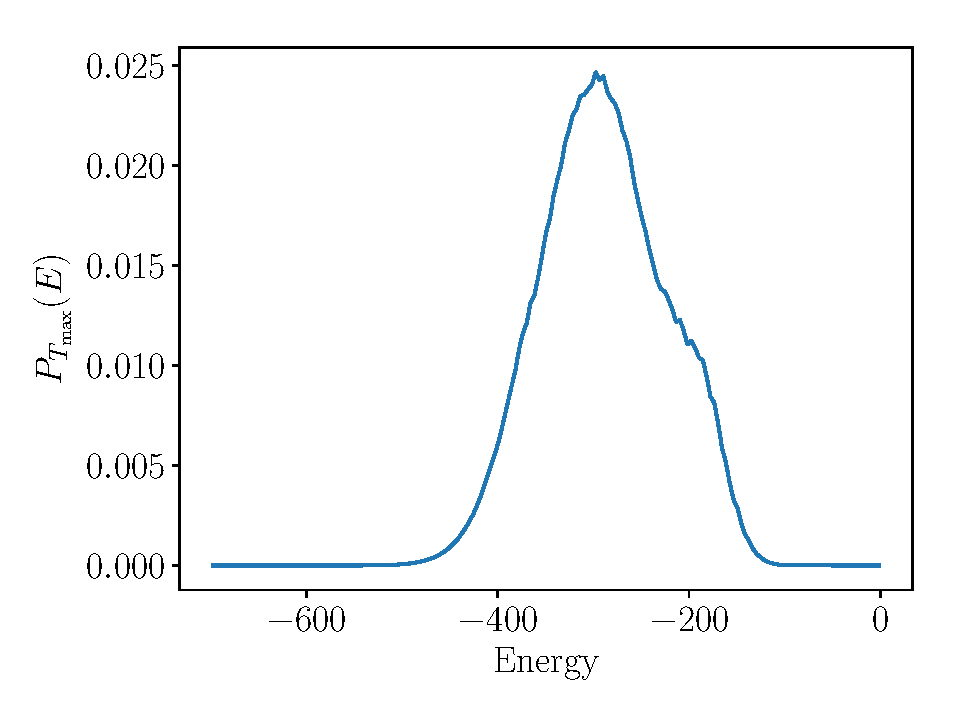
\includegraphics[width=0.49\linewidth]{projA_2.pdf}
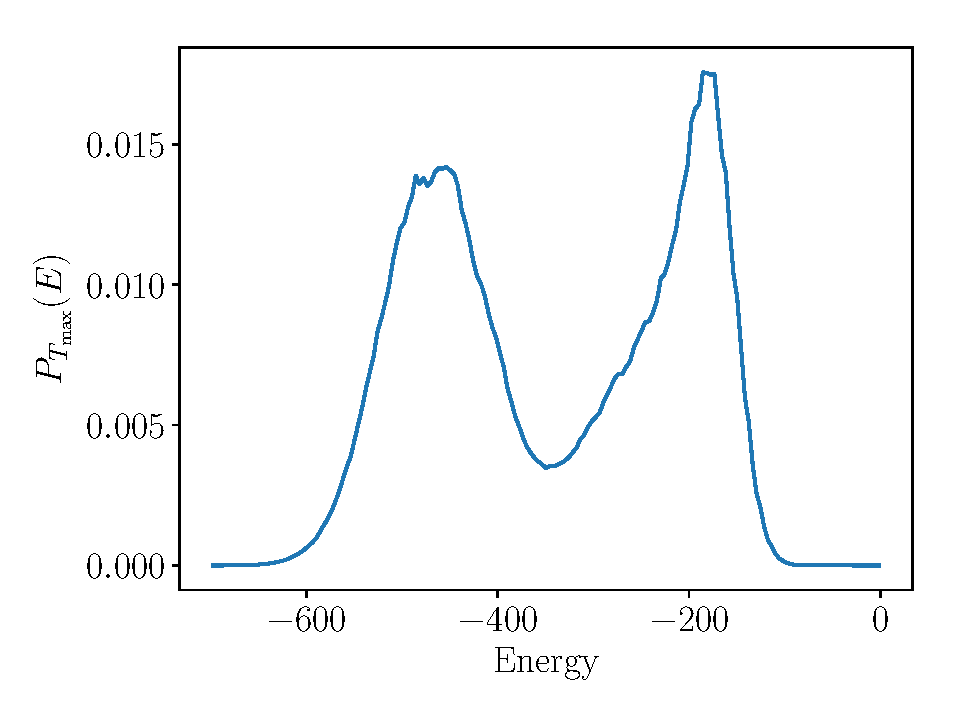
\includegraphics[width=0.49\linewidth]{projB_2.pdf}
\caption{Probability distributions at maximum temperatures for system A (left)
and B (right).}
\label{fig:pdf}
\end{figure}
\end{document}
